\section{Photometric Value Calculation}
%Výpočet mnohonásobných odrazů, algoritmus - odrazy
To evaluate the lighting system's quality of the model room in terms of standard \cite{12464} four parameters have to be observed listed in section~\ref{sec:design}. In this project only uniformity and illuminance will be used. Uniformity $U_{0}$ is calculated by the following equation:

\begin{equation}
U_{0}=\frac{E_{min}}{\overline{E}} \quad \mathrm{(-;lx,lx)}
\end{equation}

where:
\begin{description}
	\item[$E_{min}$] is the minimum illuminance of the working plane,
	\item[$\overline{E}$] is the average illuminance of the working plane.
\end{description}

Illuminances can be acquired by measurements or calculations in certain points of working planes that are chosen in accordance to the purpose of the room. To calculate the illuminance in a given point of the working plane contributions of all light sources illuminating the given point have to be summed up. This can be achieved by using luminous intensities of all the light sources pointing from the light source towards the point (Fig~\ref{fig:osv}):

\begin{equation}
E_{P\rho}=\sum_{i} \frac{I_{C \gamma i} \cdot \cos{\beta_{i}}}{{l_{i}}^{2}} \quad \mathrm{(lx;cd,-,m^{2})}
\label{eq:illSum}
\end{equation}

where:
\begin{description}
	\item[$I_{C \gamma i}$] is the luminous intensity of the light source pointing towards point P of plane $\rho$, i.e. luminous intensity of plane C at angle $\gamma$ ($C-\gamma$ angular coordinate system),
	\item[$\beta_{i}$] is the angle between the normal of plane $\rho$ and the light ray from light source $S_{i}$,
	\item[$l_{i}$] is the distance of point $P$ from the light source.
\end{description}

\begin{figure}[htb]
  \centering
  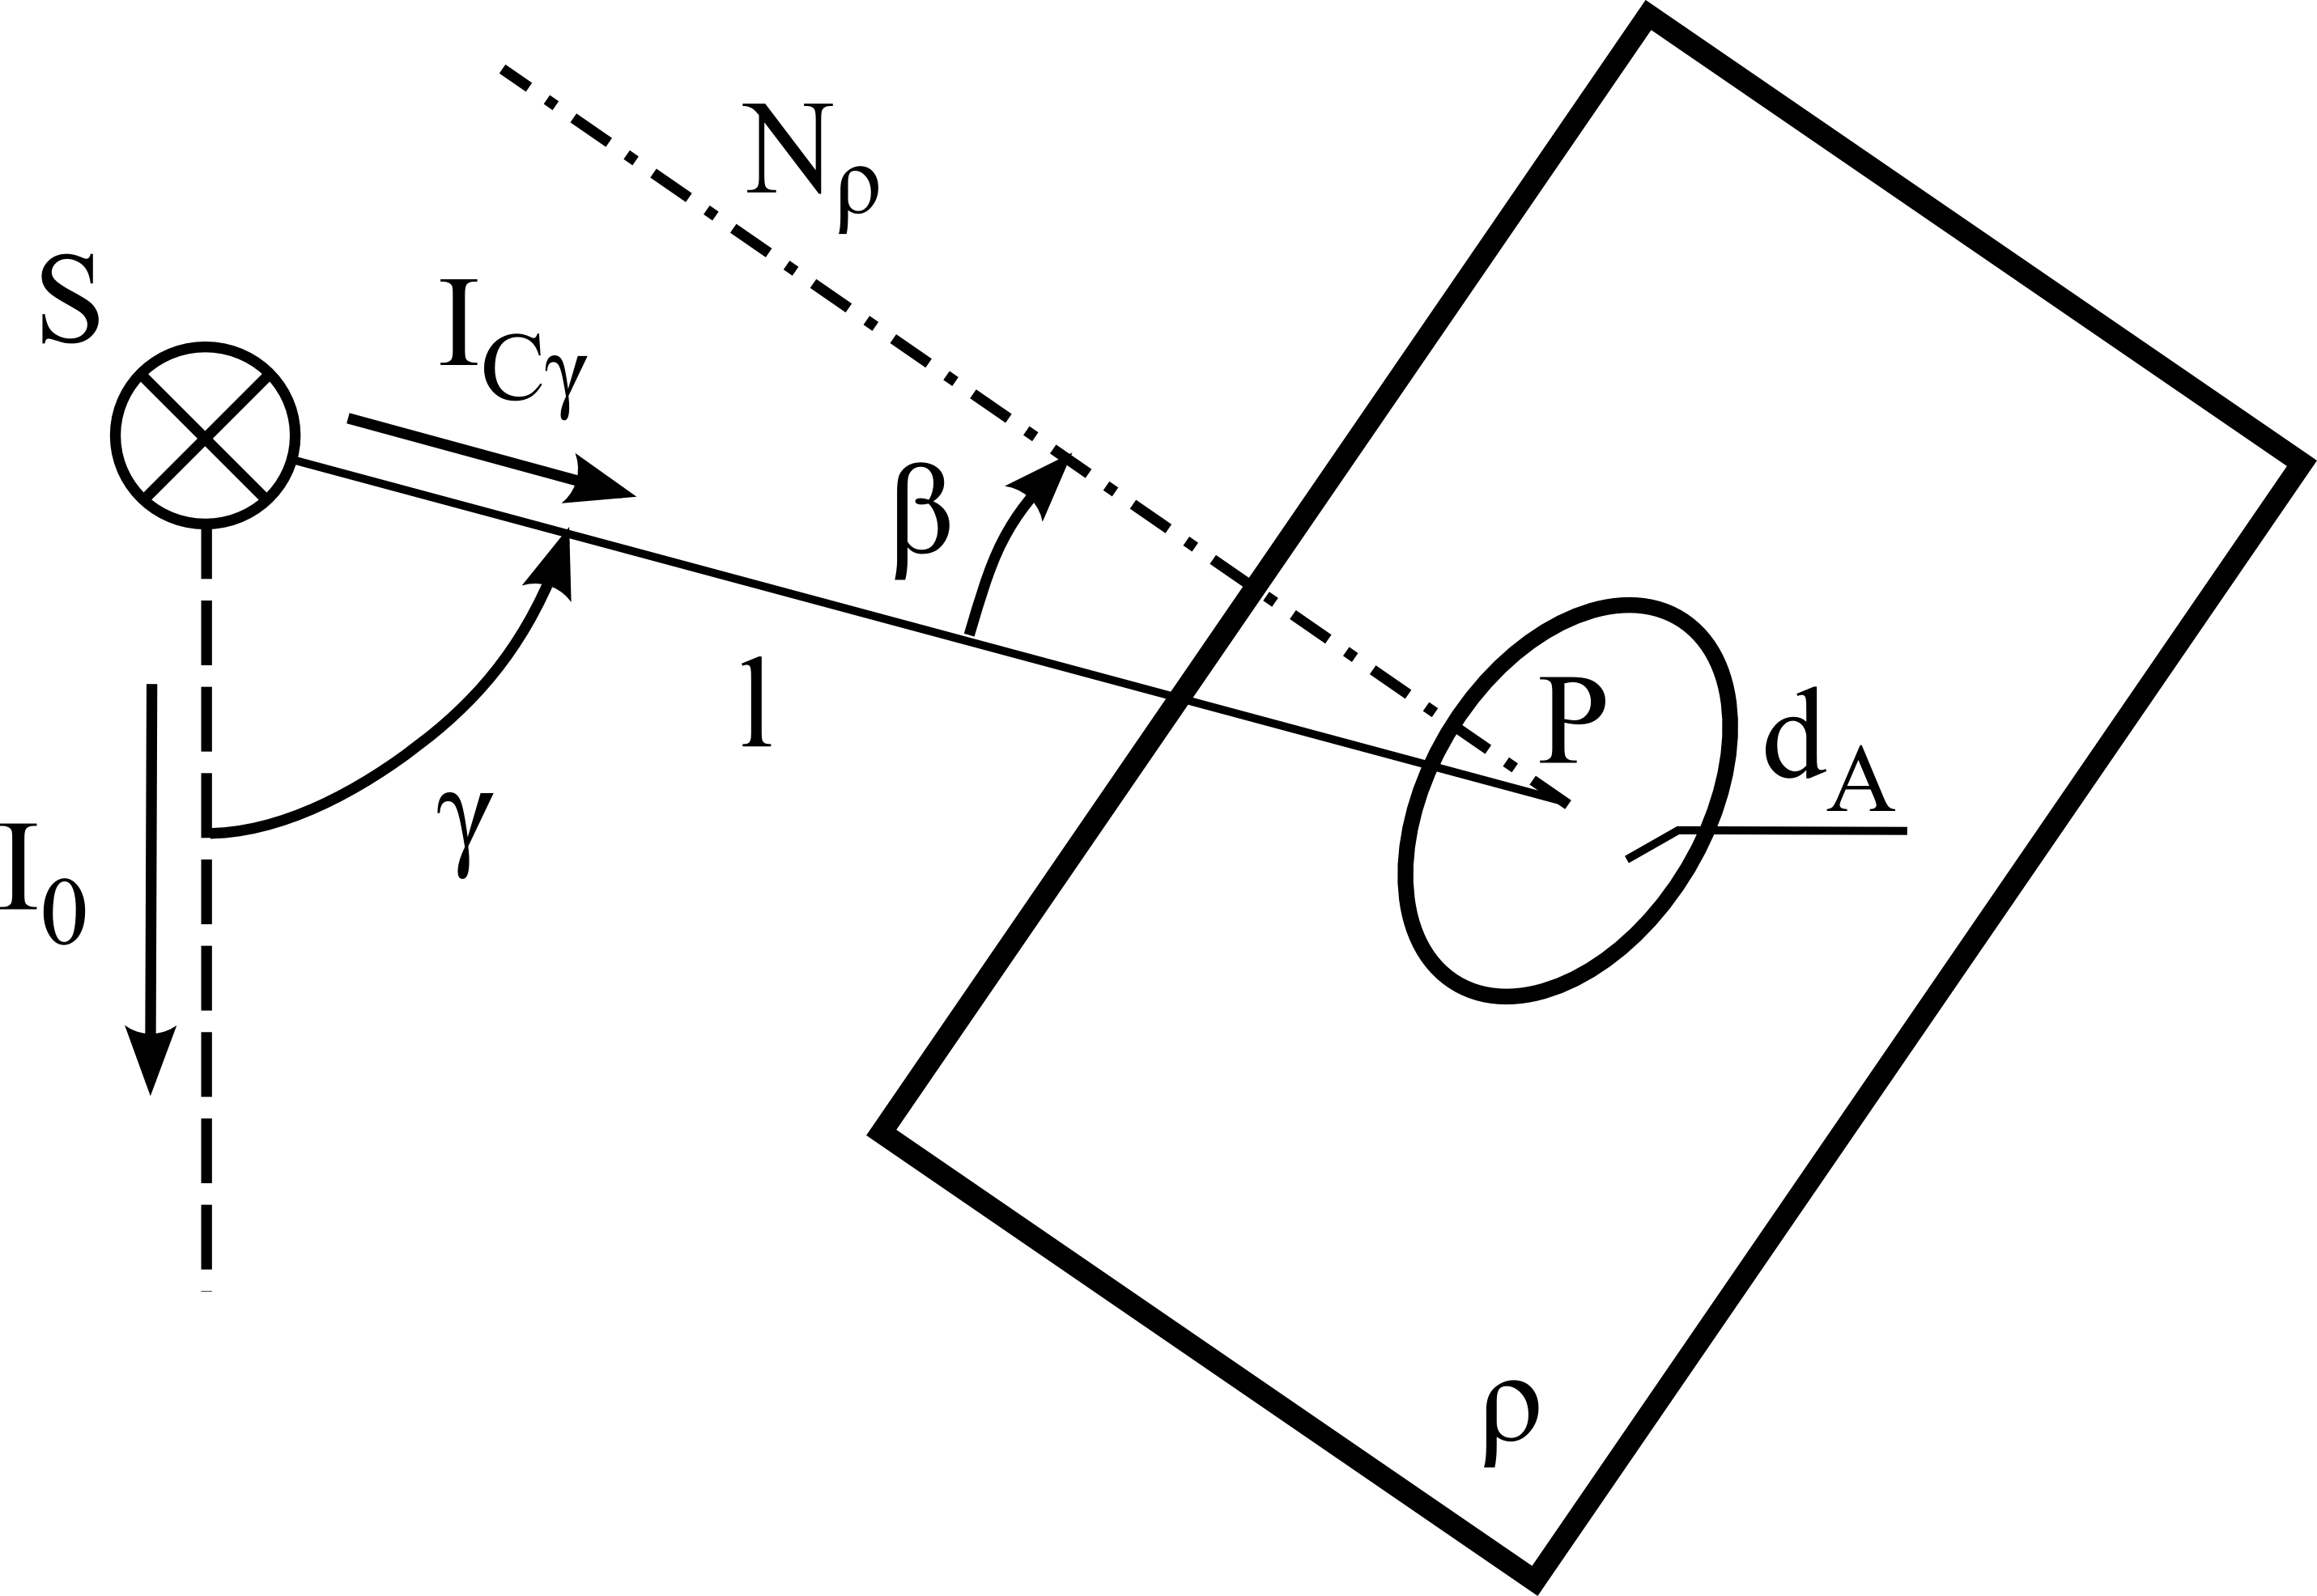
\includegraphics[width=160pt]{315_osvetlenost_bodovym_zdrojem_2}
  \caption{Light source $S$ illuminates point P of plane $\rho$.}
  \label{fig:osv}
\end{figure}

Luminous intensity curves are stored in eulumdat files supplied with luminaires to make light scene calculations possible. For most indoor luminaires the $C-\gamma$ angular coordinate system is used (Fig.~\ref{fig:cgamma}).

\begin{figure}[htb]
  \centering
  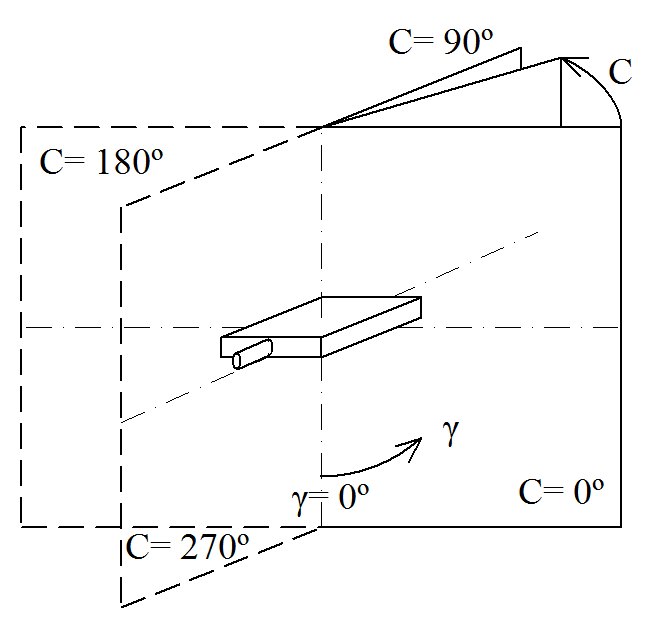
\includegraphics[width=150pt]{Cgama}
  \caption{$C-\gamma$ polar coordinate system with luminaire in center.}
  \label{fig:cgamma}
\end{figure}

To achieve more accurate simulation results of light scenes, reflections have to be included. From point's P point of view (Fig.~\ref{fig:osv}), walls, ceiling and floor will become light sources of reflected light. Using the finite element method, surfaces of the model room will be divided into smaller facets. These facets, after illuminated, will become secondary light sources (Fig.~\ref{fig:difRefl}). The process of reflections can be repeated as many times as needed. During each reflection a portion of the incident luminous flux is consumed by the illuminated surface as defined by its reflectance. Therefore after several reflections the reflected luminous flux becomes negligible.

\begin{figure}[htb]
  \centering
  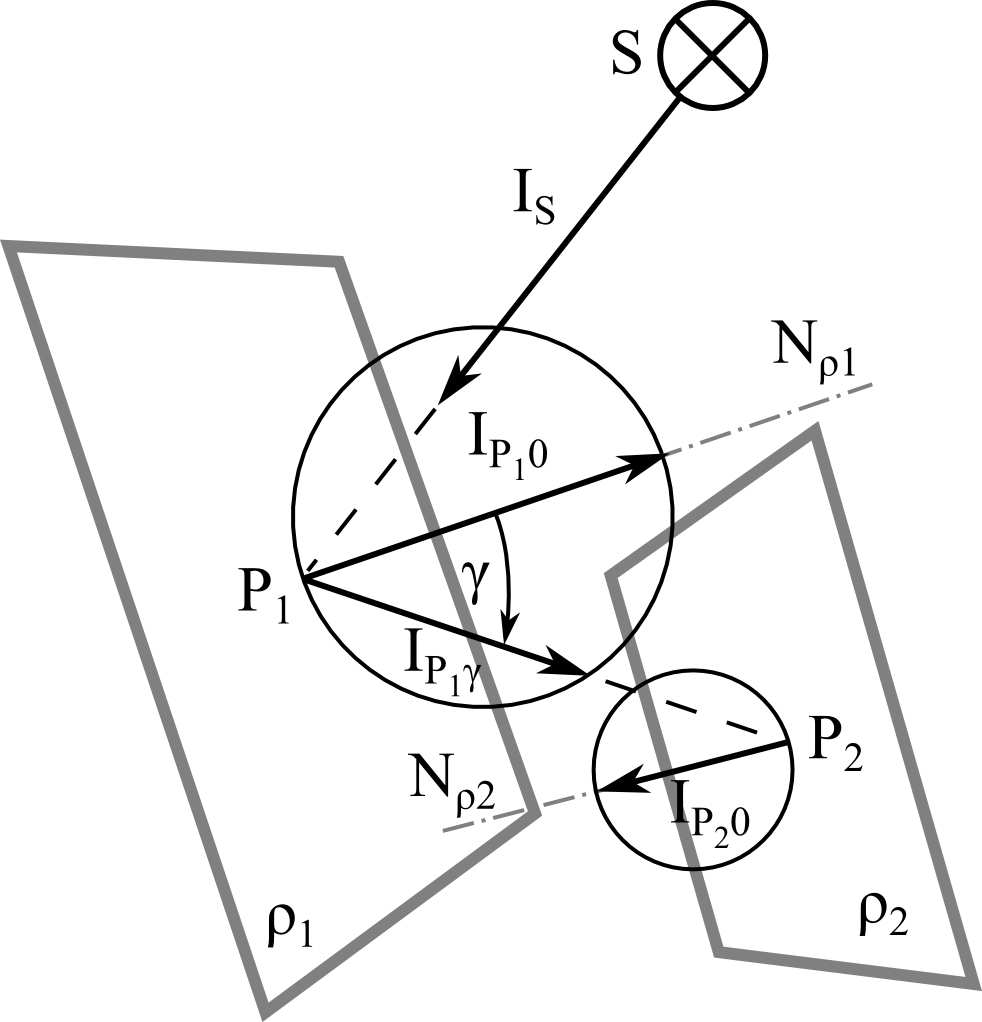
\includegraphics[width=136pt]{diffuseReflection}
  \caption{Multiple reflections between planes $\rho1$ and $\rho2$ with Lambertian reflectance.}
  \label{fig:difRefl}
\end{figure}

Most common wall and ceiling paints exhibit near Lambertian reflectance properties (Fig.~\ref{fig:difRefl}), meaning that the spacial luminous intensity distribution curve of the facet will only depend on angle~$\beta$, being the angle between the facet's normal $N_{\rho}$ and the line of center points of both facets. The model room's surfaces, including the floor, have been chosen to exhibit purely Lambertian reflectance.

After a facet has been illuminated by primary light sources and all the illuminances have been summed up (equation~\ref{eq:illSum}), the facet becomes a Lambertian secondary light source of luminous intensity \cite{Habel}:

\begin{equation}
I_{0}=\frac{\rho \cdot E \cdot dA}{\pi} \quad \mathrm{(cd;-,lx,m^{2})}
\label{eq:lumInt}
\end{equation}

where:
\begin{description}
	\item[$I_{0}$] is the luminous intensity of the facet in direction of the facet's normal,
	\item[$\rho$] is the facet's integral reflectance,
	\item[$E$] is the facet's illuminance,
	\item[$dA$] is the facet's area.
\end{description}

After obtaining $I_{0}$, the luminous intensity curve of a facet of Lambertian reflectance will be:

\begin{equation}
I_{\gamma}=I_{0} \cdot \cos(\gamma) \quad \mathrm{(cd;cd,-)}
\end{equation}

where:
\begin{description}
	\item[$I_{\gamma}$] is the luminous intensity in direction $\gamma$,
	\item[$I_{0}$] is the luminous intensity in direction of facet's normal,
	\item[$\gamma$] is the angle between the facet's normal and the line of center points of the source and destination facet.
\end{description}